\chapter{Practical Deployment for Interactive Simulations}
\label{chp:deployment}

This final technical chapter focuses on the issues surrounding the
deployment of Simulation Assisted Visual Systems (SAVS). The
organization of this chapter is divided into two main parts. First,
there will be a short review of the high level technical concerns
regarding deployment. Second, the developmental history of our
benchmark surgical application will be described, highlighting the
choices, and their rationals, made along the way.

\section{Deployment Issues}

At a high level, there are many decisions involving technology that
need to be addressed when deploying large systems. In this section,
we'll briefly look at three of the most critical for our benchmark
application: Remote architectures, Platforms, and Maintenance.

\paragraph{Network Architectures}~ One of the largest architectural
questions we need to answer is whether we want a wholly local
application or a networked application. The advantages of a local
application include decreased complexity, potentially better access to
client resources, and more control over data. Unfortunately, local
applications are also completely dependent on local resources. For
simulations, which are computationally intensive, a purely local
application might be difficult to deploy at scale due to hardware
costs. The addition of networking allows us to break many of these
issues apart and distribute them more fairly across multiple
machines. In such an architecture, servers capable of large
computations could service multiple clients, enabling larger
deployments with less capital investment. On the other hand, network
designs become dependent on another system: The network itself. For
locations with poor network connectivity, such as in the developing
world, local installations might be more valuable, despite the up
front costs.

\paragraph{Platforms}~ Platform support is another important
concern. Currently there are many popular consumer facing application
platforms. The application platform, which is often simply the
computer's operating system, defines what features and services are
available to the application. We have many choices in choosing these
platforms, depending on the device we which to run
our simulation system on. For the personal computer, operating systems such as
Microsoft's Windows, Apple's OSX, and multiple distributions of Linux,
can fulfill the role of the application platform. On smaller devices,
such as phones and tablets, Apple's iOS and Google's Android are
extremely popular choices. Finally, the Internet itself, through the
combination of HTML and Javascript on web browsers has become a de
facto operating system for many people.

Interestingly, all of these platforms, despite their differences,
support the user interface technologies (user input, 2D and 3D
rendering) required for surgical simulation
applications. Unfortunately, not all of these platforms (when
considering the operating system and device combined) can support the
computational requirements we require. This presents a curious
situation where it is possible to develop cross platform user
interfaces, but not necessarily cross platform simulations. As we'll
see later, dividing these responsibilities allows for more flexible
architectural solutions.

\paragraph{Maintenance}~ One final technical issue is the concept of
updating and maintenance. Despite the focus of deployment in this
chapter, it is important to remember that there are plenty of ongoing
research questions regarding simulation, surgical or
otherwise. Investigations of these questions might result in new
requirements for hardware or software environments. Inevitably, the
simulation system we are attempting to deploy, and possibly the
underlying platform itself, will need to be updated - whether to support a
new simulation technique or to fix more mundane bugs. When this
situation occurs, the method of deployment can greatly affect the ease
of this process. Local applications can be the hardest to manage under
these circumstances, since they are by nature decentralized and might
require wide scale hardware upgrades. Network based deployments, where
the simulation is run on remote servers, offer more opportunities for
more centralized upgrades.

\section{System Architecture Comparisons}

Over the several years of research leading up to this dissertation,
multiple system designs for a surgical SAVS were developed and
tested. In this section, each design will be covered in detail along
with its particular benefits and problems. The goal of this section is
to demonstrate how different system designs fit with different
deployment concerns and how emerging technologies can support
simulation deployments more easily than in the past.

The core feature set for all implementations, which was defined
through conversations with our domain collaborators including
Dr. Court Cutting, is described below.

\begin{enumerate}
\item \textbf{Real-time physics simulation} 3D models of tissue were
  simulated via an embedding lattice deformer design, allowing users
  interactive visualizations of physical responses. Multiple models
  were made available for simulation, ranging from more academic
  shapes designed to illustrate particular principles to a more
  realistic model of the human scalp. 

 \item \textbf{Keyboard and Mouse Interface} Users were presented with an
   open 3D space which contained the actively simulated model. They
   were allowed to move the virtual camera through the space using
   their keyboard and mouse. Additionally, tools (such as a virtual
   scalpel and virtual sutures) were made available via a simple
   ``click and place'' interface.
  
\item \textbf{Local Flap Operations} All models represented a 2.5D
  (generally a thin, possibly curved, sheet) region of tissue with a
  defined top and bottom side. Intended operations were ``local
  flaps'', where simulated tissue was cut and moved
  around in a local region for the purposes of closing holes or
  relieving stress patterns.

  \item \textbf{Free Form Cutting} Incisions were placed into
  tissue via line segments drawn on the top surface of models. Cuts
  were allowed to be defined with arbitrary complexity, including the
  isolation and removal of regions, with the only restriction that
  they all be performed all at once, before simulation began.

  \item \textbf{User Interactions} Users were allowed to interact with
    the running simulation via force constraints. These constraints
    took the form of ``hooks'', positional constraints that pulled
    simulated material towards a point in space, and ``sutures''
    double ended constraints that pulled one region of simulated
    tissue towards another region.

  \item \textbf{Operation Recording/Playback} Users were allowed to
    record sequences of operations and then play them back on
    subsequent run throughs. This functionality was designed to
    replace the more traditional approach of drawing operation steps
    in textbooks.
    
  \end{enumerate}


  The tool's user interface was proscribed and prototyped by our
  primary domain collaborator, Dr. Court Cutting. The choices made in
  the process of designing the interface were made in response to the
  background and familiarity to three dimensional modeling tools of
  our expected user base, plastic surgeons.  

  
  % Before moving on to the specific details of each implementation,
  % some time should be spent breaking these systems down according to
  % SAVS aspects, as detailed in Chapter \ref{chp:motivation}. In
  % terms of Geometry, all of the designs presented in this chapter
  % presented a three dimensional object to the user via a standard
  % computer display, which represented either a real anatomical region
  % (i.e. the human scalp) or a conceptual workspace for academic
  % examples. There was minimal or no surrounding environment around the
  % simulated tissue object. The system was Reactive to users by means
  % of both user constraints and by supporting topology alteration,
  % allowing them to push, pull, and cut the virtual tissue. Dynamism
  % was provided by a continuous quasistatic simulation, which used
  % successive frames of iteration to deliver time-evolving deformations
  % as users interacted with the object. Direct user Interaction came in
  % the form of placing point constraints, either from the object to
  % fixed locations in space or to another point on the object, and by
  % drawing incisions with C0 continuous curves. Finally, the systems
  % provided Utility for training and authoring by supporting loading
  % and saving of procedures, along with interactive simulation rates to
  % support real-time authoring applications.

\subsection{Traditional Desktop Application: Building the Monolith}

The first design approach followed that of many traditional native desktop
applications. All components of the application were compiled together
as a single binary executable which ran on a single machine. This
initial design used C++ as the development language, both for the
underlying simulation engine and for the graphical user
interface. This approach had many positive aspects:

\begin{enumerate}
  \item \textbf{Single Development Language} By using one language for
    all components, building APIs was made considerably easier, which
    facilitated faster development.

  \item \textbf{Integrated Application} Since the entire application
    was linked as a self-contained binary, it was easy to setup and
    run. External dependencies amounted to several libraries required
    for the graphical interface and OpenGL graphics.

  \item \textbf{Accelerator Access} By running entirely on a single
    machine, the simulation engine had access to all computational
    resources on the client, including all CPU cores and available
    accelerator cards. In the latter case, MPI was used to communicate
    with installed Intel Phi accelerators\footnote{This unfortunately
      broke the ``self-contained binary'' aspect of this design, as
      the MPI routines required multiple processes running on
      different physical nodes. However, since the MPI enabled
      application could be launched via the standard ``mpirun'' command, it
      still resembled a self contained application.}. 

   \item \textbf{Fully Featured Graphics Stack} Running as a native
     application, this design had access to the full OpenGL 4.0
     specification. This allowed it to be developed with modern OpenGL
     techniques.

   \item \textbf{Platform Control} Since everything was designed by
     hand, all aspects of the application could be tuned to desired
     functionality. While certain choices were constrained by
     selection of a GUI toolkit library ~\citep{wxWid:2017}, the choice of the
     library itself was made freely.
    
\end{enumerate}

 In total, these aspects made for a well-performing client, capable of
 running optimized simulation code and displaying a functional visual
 interface for the surgical simulation. Unfortunately, it had several
 drawbacks that ultimately made it a poor choice for future
 development:

 \begin{enumerate}

   \item \textbf{Lack of Cross Platform} Due to it being designed
     purely with native C++ code, moving to new platforms was
     exceedingly difficult. For desktop operating systems, such as
     Windows and OSX, switching was a matter of recompiling and
     working out platform incompatibilities. The choice of wxWidgets as
     a GUI toolkit library helped in this regard, but for more mobile
     platforms, like iOS, Android, or HTML, there were no options.   
   
   \item \textbf{Complex GUI Development} While the GUI library,
     wxWidgets, was chosen for its cross platform capabilities, it was
     not especially friendly towards rapid development of useful user
     interfaces. As such, the GUI was rather difficult to use and hard
     to modify.

   \item \textbf{Scalability Concerns} The design's primary strength -
     a self contained application, was also its largest drawback for
     deployment. By executing on a single workstation, it required an
     entire workstation per instance. This was unpalatable for larger
     installations, such as a classroom setting, where few institutions
     could or would be willing to buy high end workstations for each student.
   
 \end{enumerate}

 
 It was this last drawback that pushed our development of the system
 in a new direction: network based simulation.

 \subsection{Network Simulation: A Three-Tiered Architecture}
 
 Unlike the previous design, the next iteration explored the potential
 of network, or cloud, based simulation. The idea was straightforward:
 it would be an architecture where simulation would be performed on a
 remote machine and its results displayed on a local client. These
 initial forays into this idea were built on top of the previous client and
 used an network interchange library from the Apache Project called
 Thrift~\citep{ASF:2008--2014}. Thrift allowed the creation of multi-language bindings to be
 delivered over network as RPC (Remote Procedure Call) APIs. Initial
 experiments involved splitting the former unified application into
 two parts: a visual frontend and a simulation backend. These parts
 were be joined together via Thrift, allowing them to communicate over
 the network.

 Once this new organization was working, the frontend was rewritten as
 a web client, which used HTML, Javascript, and WebGL~\citep{webgl1.0}
 to replicate the functionality of the older C++ GUI. Further
 experimentation with this arrangement eventually showed a significant
 problem with Thrift: it made developing smooth, lag-free user
 interfaces somewhat tricky. The fault primarily laid with Thrift's
 RPC style conventions. Under this communication style, a client would
 continuously poll the server for new information. Under a multiple
 client scenario, this method broke down, causing unnecessary network
 traffic and lag.  This issue caused us to seek a new communication
 method, one that could support a ``push'' style communication. We
 finally settled on a newer Web standard: Websockets.

 The Websocket standard~\citep{rfc6455} is a full-duplex communication protocol
 available in HTML5. The standard defines a custom protocol over TCP, where
 messages can be sent from either end and are guaranteed to
 arrive in order on the other side. The primary benefits of the
 protocol are easy bidirectional communication and low overhead. Since
 the protocol uses a custom TCP-based protocol instead of HTTP, it can
 operate without unnecessary headers and transmit data as byte streams.
 Replacing Thrift with Websockets was the final piece of what was
 later referred to as our Three-Tiered Architecture.


\begin{figure}[t]
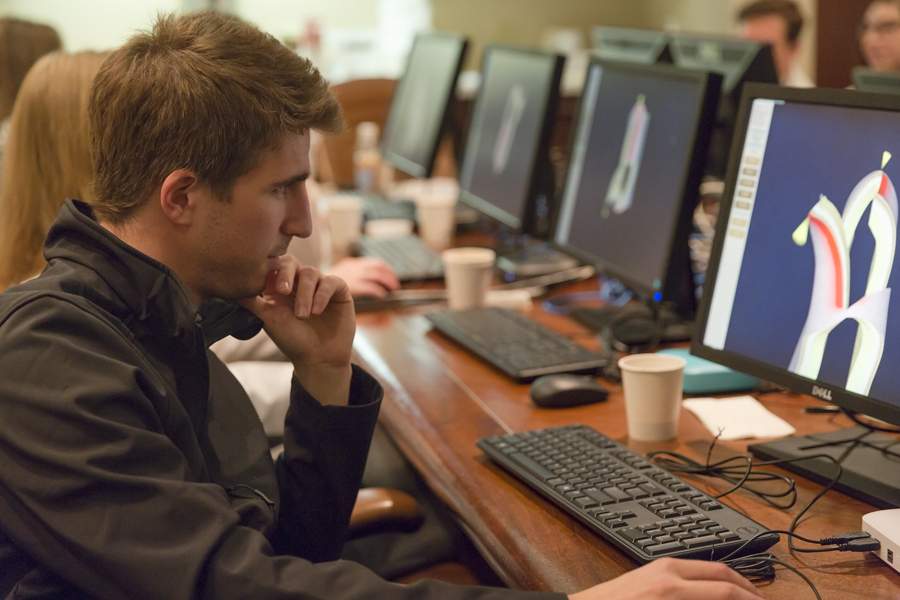
\includegraphics[width=\columnwidth]{chapter_gridiron/images/CS_SurgerySim.jpg}

%\caption{Pilot deployment of our interactive simulation system. A group of 14 MD residents in a program for plastic and reconstructive surgery interact and experiment with our platform. The simulator front end runs as a web-based application on ChromeBox\copyright clients, while numerical simulation occurs on a central server platform.} 
\caption{Pilot deployment of web-based simulator}{Pilot deployment of
  our interactive web-based simulator with 14 Plastic \&
  Reconstructive Surgery medical residents at the University of
  Wisconsin-Madison. This demo used the second architecture, the
  three-tiered design.}

\label{fig:pilot}
\end{figure}
 
 The three-tier design consisted of the following components: a
 web-based client (Tier 1), an SMP server for modeling (Tier 2), and a
 many-core accelerator for numerics (Tier 3).  The \emph{front-end
   client} served primarily as the user interface to the system. The
 client was responsible for acquiring user input and visualizing the
 simulation results. Communication is performed via the WebSockets
 standard, which allows the client to operate under a push data
 model. Thus, the remote server could send updates to clients when
 they become available instead of requiring clients to poll for
 updates.
 
 We refer to the \emph{second-tier platform} as the CPU host. Its
 primary task was to perform all non-simulation computation that can
 be offloaded from the client level. The host manages user sessions,
 stores and loads scene data from disk, performs geometric
 manipulations (non-manifold meshing and incision modeling) as a
 result of user actions and runs collision detection. This tier
 requires large amounts of memory, beyond what is natively offered on
 a GPU or Many-Core accelerator. The \emph{third tier} is the
 numerical solver, which executes all low-level compute intensive
 kernels (but not combinatorial tasks such as mesh generation). We
 have implementations that allow this layer to either run on the same
 CPU platform as the 2nd-tier code or run natively on a Xeon Phi
 accelerator, interfacing with the host over MPI. This later
 functionality is similar to how the initial monolithic system design
 functioned.

 The specific benefits from this design approach were:

 \begin{enumerate}
   \item \textbf{Fast GUI Development} As the final implementation of
     the frontend was written in HTML and Javascript, iteration on the
     GUI was much faster due to visual debugging tools and more mature
     support libraries for web application development.

   \item \textbf{Native Support for Network Simulation} Since the
     frontend was designed as a web application, by nessessity it
     needed to connect to the simulation engine via network
     protocols. By using Websockets, we were able to construct a
     server side implementation that could broadcast the current
     simulation state to multiple connected clients
     simultaneously. This allowed for centralized simulation and more
     scalable deployments.

   \item \textbf{Cross Platform Support} While the simulation engine
     was still using native code, and required additional effort to
     port to other platforms, the HTML frontend was able to run on
     multiple platforms and form factors with minimal development
     effort. We were able to successfully deploy the client on
     desktops, tablets, and smartphones. Since the client's
     computational responsibilities were limited, it could be run a
     wide range of hardware as long as it had a reasonably moderate
     graphics accelerator.

   \item \textbf{Service Integration} Finally, a side benefit of the
     Web application frontend was the possibility of integration with
     other web services. For production deployment, this would allow
     easier connection with existing web authentication platforms and
     online help desk services. 
     
 \end{enumerate}


 However, no design is perfect. Like the previous monolithic design,
 the three-tiered design had several drawbacks:


 \begin{enumerate}

   \item \textbf{Complex Infrastructure} While it was praised earlier,
     there is no denying there exists added difficultly when deploying
     and running a network application that must coordinate between
     multiple independent nodes. This is the unfortunate double edged
     sword aspect of any network or cloud service.

   \item \textbf{Network Bandwidth Dependency} Unlike video games,
     where visual assets are typically cached on clients and then
     modified according to predetermined scripts, the geometry of
     deformable simulations is inherently unpredictable by the
     client. As such, every frame of the simulation requires
     transmitting all of the deformation data down to the client. For
     low polygon models this is manageable, but highly detailed
     biological scenes can require significant amounts of network
     bandwidth, or they risk causing unacceptable lag for clients.

     % \item \textbf{Privacy Risks} As mentioned earlier, transmitting
     %   patient specific data over the network can introduce privacy
     %   dangers that run afoul of legal restrictions.

     \item \textbf{Loss of Platform Control} While using a web client
       provides a large amount of cross platform support, it places
       the client at the mercy of the web browsers that are running
       it. One of the primary challenges facing web developers is the
       number of small differences between browsers (and versions)
       that can sometimes mean the difference between a working client
       and a failing one.

     \item \textbf{WebGL Only} While the WebGL standard contains most
       of the features that the modern OpenGL standards support, there
       are gaps and differences in functionality. However, as more and
       more 3D applications find their way onto the Web, these
       standards are becoming more and more robust.
     
 \end{enumerate}

 To evaluate this design, we conducted a pilot deployment for the
 medical residents in the University of Wisconsin-Madison Plastic \&
 Reconstructive Surgery program, as part of a workshop on craniofacial
 reconstruction techniques. We set up a local switched network at the
 location of the workshop, with a portable desktop-grade computer
 (with a 4-core Intel 4770R processor and 16GB RAM) acting as the Tier
 2/3 simulation server, and a collection of eight Chromebox web-based
 thin clients as the user stations (our setup can be seen in Figure
 \ref{fig:pilot}). Although our modest portable server did not have
 the computing power available to our many-core accelerated server
 systems which we used for our large-scale offline simulations, its
 (AVX-accelerated) performance was more than adequate to deliver an
 interactive user experience. Total cost of the entire deployment,
 including server, networking and client stations was \$4,000.

  Participants were initially given an extremely brief orientation on
  visual navigation within the application and its interface. In first
  part of the deployment exercise, the workshop instructor (a seasoned
  user of the system) authored several different reconstructive
  procedures on different anatomical models, while the participants
  were invited to follow the manipulations as they were taking place
  (without affecting them) by adjusting the view of the dynamic model
  on their own station. Subsequently, individual participants who had
  no prior exposure to the system were invited to drive the authoring
  process, which their colleagues would virtually follow. The workshop
  instructor provided guidance on clinical aspects of the repair being
  authored, while questions about the user interface would be recorded
  and addressed by the system developers. At the conclusion of the
  exercise, the participants were debriefed and given the opportunity
  to evaluate their experience and propose improvements.

  While this approach proved successful and provided many nice
  benefits for developers, it did so at the cost of added complexity
  nearly all cloud based systems create. The difficulties of managing
  a distributed system, both in development and for the potential to
  be deployed in areas with unreliable networks, inspired the third
  design approach, which attempted to combine the benefits of the two
  prior architectures.
 
 \subsection{Monolithic Web Design: Electron}

 The third design made use of a relatively recent framework called
 Electron. Electron~\citep{Electron:2016} is a framework for building
 traditional desktop applications by using web application development
 tools. It does so by combining Google's open source browser Chromium
 and NodeJS~\citep{NodeJS:2017}, an interpreter and set of standard libraries for
 Javascript which allow more traditional system level calls, such as
 file access and process management. This framework provides
 developers access to a familiar web development environment, along
 with access to the underlying operating system, functionality
 normally inaccessible in the browser. Using this framework, it was
 possible to build the third design architecture: the monolithic web
 application.

 The primary concern with using Electron as a the application
 framework is performance. With the original design, everything was
 written with native code, which allowed for optimized code to
 implemented with appropriate care. The second design ran a native
 code simulation server, providing effectively the same benefits over
 the network. For the Electron based design, a different approach was
 required. In order to maintain native performance where it was most
 needed, the simulation engine was repackaged into a native NodeJS
 extension. Using the API provided by V8, the underlying Javascript
 interpreter for both Chromium and NodeJS, the native C++ code was
 exposed to the higher level Javascript code. From the Javascript
 environment, the C++ code could be called just like other Javascript
 routines, except with native performance - they were able to use all
 of the multithreading and SIMD optimizations described in previous
 chapters.

 With this native wrapping completed, the rest of the application
 could be ported over from the second architecture design in a
 straightforward fashion. The web client code required minimal
 changes, since it was still running in a web browser like before. The
 only new code required was a re-implementation of the connection
 between the client and the simulation engine. This was again done
 with Websockets, only this time as connections entirely internal to
 the application. This was a conscious choice - allowing for a
 potential client-server mode in the future. This design successfully
 merged the major positive characteristics from the previous two
 designs: an integrated desktop application, access to local
 computational resources, faster user interface development, and easy
 access to network simulation. The major drawbacks of this design were
 the added complexity of the multi-language bindings and a dependency
 on the Electron framework\footnote{However, since we are now only
   targeting a single web browser, the one bundled with Electron, we
   are freed from worrying about supporting multiple browser versions.}. 

 
%%% Local Variables:
%%% mode: latex
%%% TeX-master: "../document"
%%% End:
